\section{装备方案评估（七种单船组合）}

\subsection{成本模型}

所有方案都包含“工作级 ROV + 水面雷达/目视”两项共有资产；三件可选装备
（深水拖曳侧扫、深水多波束、AUV）做非空组合，共 $2^3-1=7$ 种方案。
单次事故（4 天）成本估计见 \tabref{tab:cost}。

\begin{table}[H]
\centering\small
\caption{单次事故成本估计（万美元；公开市场量级估计）}
\label{tab:cost}
\begin{tabular}{@{}lrrrr@{}}
\toprule
项目 & 固定/动员 & 每天 & 4 天合计 & 说明\\
\midrule
水面雷达/目视 & 0 & 3 & 12 & 母船已有\\
深水拖曳侧扫 & 10 & 2 & 18 & 拖鱼+绞车+操作员\\
深水多波束 (WCI) & 20 & 8 & 52 & 船载多波束+处理\\
AUV & 25 & 8 & 57 & 2000 m 级 AUV\\
工作级 ROV & 40 & 15 & 100 & 含母船船时与人员\\
\midrule
共有项小计 & — & — & 112 & 雷达 + ROV\\
增加侧扫 & — & — & +18 & \\
增加多波束 & — & — & +52 & \\
增加 AUV & — & — & +57 & \\
\bottomrule
\end{tabular}
\end{table}

\subsection{七种方案的结果}

\begin{table}[H]
\centering\small
\caption{7 种单船装备组合的搜索结果（30\,000 粒子，$t=0$ 立即搜救）}
\label{tab:schemes}
\begin{tabular}{@{}llrrrrrrr@{}}
\toprule
编号 & 组合 & 成本 & $P_{24}$ & $P_{48}$ & $P_{72}$ & $P_{96}$
& $T_{50}$ (h) & $\mathbb E[T]$ (h)\\
\midrule
M1 & 侧扫 & 130 & 0.364 & 0.376 & \textbf{0.382} & 0.388 & $>$96 & 61.4\\
M2 & 多波束 & 164 & 0.812 & 0.847 & \textbf{0.865} & 0.877 & 3 & 18.1\\
M3 & AUV & 169 & 0.718 & 0.767 & \textbf{0.789} & 0.803 & 5 & 26.8\\
M4 & 侧扫+多波束 & 182 & 0.849 & 0.880 & \textbf{0.896} & 0.905 & 3 & 15.0\\
M5 & 侧扫+AUV & 187 & 0.788 & 0.827 & \textbf{0.845} & 0.858 & 4 & 21.0\\
M6 & 多波束+AUV & 221 & 0.902 & 0.930 & \textbf{0.943} & 0.951 & 3 & 10.4\\
M7 & 侧扫+多波束+AUV & 239 & 0.920 & 0.945 & \textbf{0.955} & 0.962 & 3 & 8.9\\
\bottomrule
\end{tabular}
\end{table}

\begin{figure}[H]
\centering
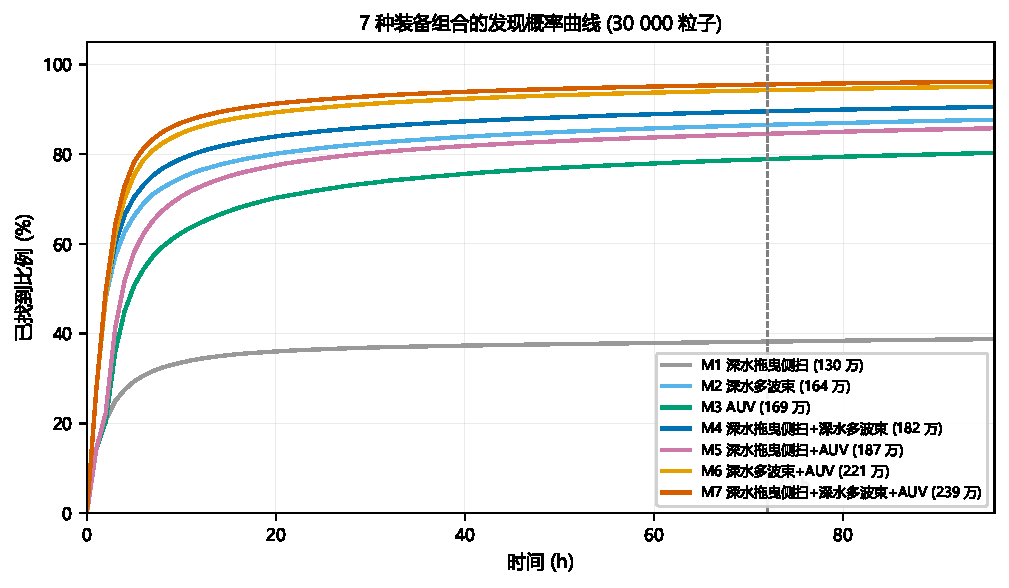
\includegraphics[width=0.68\textwidth]{fig_search_curves}
\caption{7 种方案的发现概率曲线 $P(t)$（虚线为 72 h）。M1（侧扫单独）在 38\% 附近
饱和，其余方案在 24--72 h 内陆续升到 85\%--96\%。}
\label{fig:schemes}
\end{figure}

\subsection{成本–效能分析}

\begin{figure}[H]
\centering
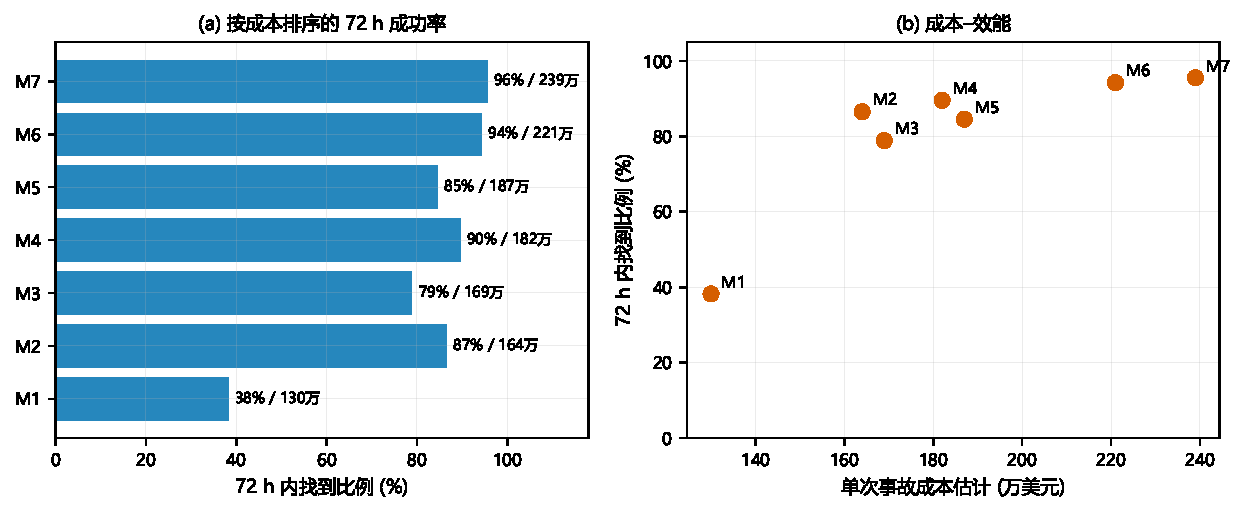
\includegraphics[width=0.68\textwidth]{fig_search_cost}
\caption{(a) 按成本排序的 72 h 成功率；(b) 成本–效能散点。拐点出现在 M4
（侧扫+多波束，182 万美元，89.6\%）。}
\label{fig:cost}
\end{figure}

\paragraph{三个结论.}
\begin{enumerate}[leftmargin=1.8em,itemsep=0pt]
\item \textbf{侧扫单独不可行}：$P_{72}=38.2\%$。原因是水柱分支占 62\%，侧扫只成像海底，
      看不到水柱目标。这是一条“装备必须匹配目标类别”的硬约束；
\item \textbf{“能搜水柱”是分水岭}：多波束（86.5\%）与 AUV（78.9\%）单独都可用，
      但都不够；两者互补（多波束快、AUV 灵活但受 2000 m 深度限制），组合 M6 达 94.3\%；
\item \textbf{成本–效能拐点是 M4}：在共有项 112 万美元之外，多花 18 万加侧扫即可把
      深水海底分支覆盖完整，$P_{72}$ 从 86.5\% 提到 89.6\%；再花 39 万加 AUV（M6）
      只多 4.7 个百分点；M7 再加侧扫仅多 1.2 个百分点，接近饱和。
\end{enumerate}

\subsection{响应延迟的影响}

实际搜救存在“失联 $\to$ 通知 $\to$ 集结 $\to$ 开始搜索”的延迟。我们把它作为参数，
对 M1/M2/M7 在 0/6/12/24 h 四档下重跑（\figref{fig:delay}）。

\begin{table}[H]
\centering\small
\caption{额外动员延迟对 $P_{72}$ 的影响（主算例）}
\label{tab:delay}
\begin{tabular}{@{}lcccc@{}}
\toprule
延迟 & 0 h & 6 h & 12 h & 24 h\\
\midrule
M1 侧扫 & 38.2\% & 29.1\% & 25.9\% & 22.4\%\\
M2 多波束 & 86.5\% & 58.4\% & 47.6\% & 35.6\%\\
M7 三件套 & 95.5\% & 73.3\% & 61.3\% & 47.4\%\\
\bottomrule
\end{tabular}
\end{table}

\begin{figure}[H]
\centering
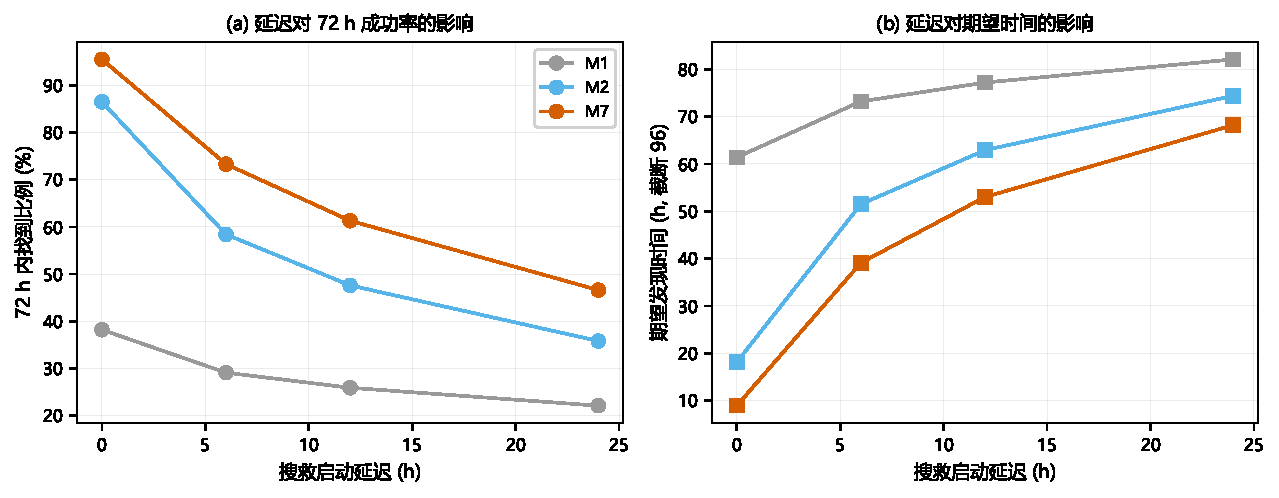
\includegraphics[width=0.66\textwidth]{fig_search_delay}
\caption{延迟对 72 h 成功率与期望发现时间的影响。延迟 6 h 就使 M2 从 86.5\% 掉到
58.4\%；M7 的冗余度最高，抗延迟能力最强。}
\label{fig:delay}
\end{figure}

延迟的杀伤力来自 $A_{95}$ 的增长：每多等 6 h，预测云面积扩大一倍以上，
而装备的覆盖能力不变。因此对运营方而言，\textbf{“待命与动员时间”应作为与装备
并列的核心指标}。
